%vim: fo-=t
\section{Android Apps}\label{sec:sota_apps}
In this section we investigate the state of the art of synchronized streaming of music between different wirelessly connected mobile devices.
We found two apps capable this:
\begin{itemize}
    \item SoundSeeder
    \item AmpMe
\end{itemize}

These apps are found by searching through sources like Google\footnote{\url{https://www.google.dk} with the search terms ``android sync music playback''}, YouTube\footnote{\url{https://www.youtube.com/} with same search terms as on Google}, and Google Play Store\footnote{\url{https://play.google.com/store}} and from recommendations on various forums.
An additional criteria for an app to be considered here is that the app must not be abandoned by the developers,
which we defined as being without an update since 2013, and being incompatible with new devices.

To clarify, Google Play Store is the official place to install or buy apps for Android.

Both of the apps use a master/slave connection and use different terms for their setup.
For clarification we generalize these terms.
We call the device which selects the music and streams it, the master, and the devices which connects to the master (SoundSeeder calls it ``Speaker''), are referred to as slaves.

\subsection{SoundSeeder}\label{subsec:soundseeder}
SoundSeeder\footnote{\url{http://soundseeder.com}} is an app made by JekApps.
The version as of \formatdate{9}{2}{2017} is 1.6.5.

It is compatible with Android 4.1 and above, for older versions of Android (2.2--4.0),
another app called \textit{SoundSeeder Speaker} makes it possible for a device to be used as a slave.

SoundSeeder also provides a Java application for compatibility with other platforms e.g. Windows, macOS and Linux, but does not support iOS and Windows Phone\cite{soundseeder_ios}.

The app consists of a top menu and a burger menu at the left side, as seen on \cref{fig:soundseeder_screenshot}.
In the burger menu, the user can choose the different playback possibilities and switch to slave mode.
The main view of the app is a music player, where the playback can be controlled.
To play music to other devices as a master, press the ``add music button'' in the top menu,
choose the source of the music and choose the preferred music, and press play.

To connect to a playing master device, as a slave, select the speaker mode from the burger menu.
If it finds the device, it connects automatically.
It can take a bit of time for the slave device to find the master device, which can seem confusing and make users think they need to connect manually with an IP address.

The process of joining, when the slave is given the time, is rather simple.
The user interface is clotted with features and menus, which makes the app hard to navigate.
The user interface of the app looks and feels outdated, i.e.\ not following the same design guidelines as newer and more popular apps.

SoundSeeder streams music via Wi-Fi,
which means that all phones have to be on the same network\cite{soundseether_faq}, it is also possible to use an ad-hoc network (Android Hotspot).
The music source of the master device can be Google Play Music, online radio stations, UPnP and DLNA devices, local media, and YouTube if using semperVidLinks\footnote{\url{https://play.google.com/store/apps/details?id=com.semperpax.sempervidlinksFree}}, an app for extracting video links.
SoundSeeder also supports streams from external sources, e.g.\ a microphone or AUX device.
The supported media formats further depend on the used master device and its Android version.\cite{soundseether_faq}

SoundSeeder synchronizes the audio playback when a slave connects, but it can also be done manually on the slave device.
On \cref{fig:soundseeder_slider}, the manual synchronization adjustment for SoundSeeder can be seen.
This slider is used in the case that the music is not fully synchronized, and goes from $-400 ms$ up to $+400 ms$, in $10 ms$ increments.
Additionally there is an auto synchronization button in the top menu and on the slider menu window.

SoundSeeder is free to install but the free version only allows two slave devices to connect for up to 15 minutes at a time.
The app license costs 39.90 DKK\@.

\begin{figure}[h!]
    \centering
    \begin{subfigure}[b]{0.45\textwidth}
        \footnotesize
        \centering
        \frame{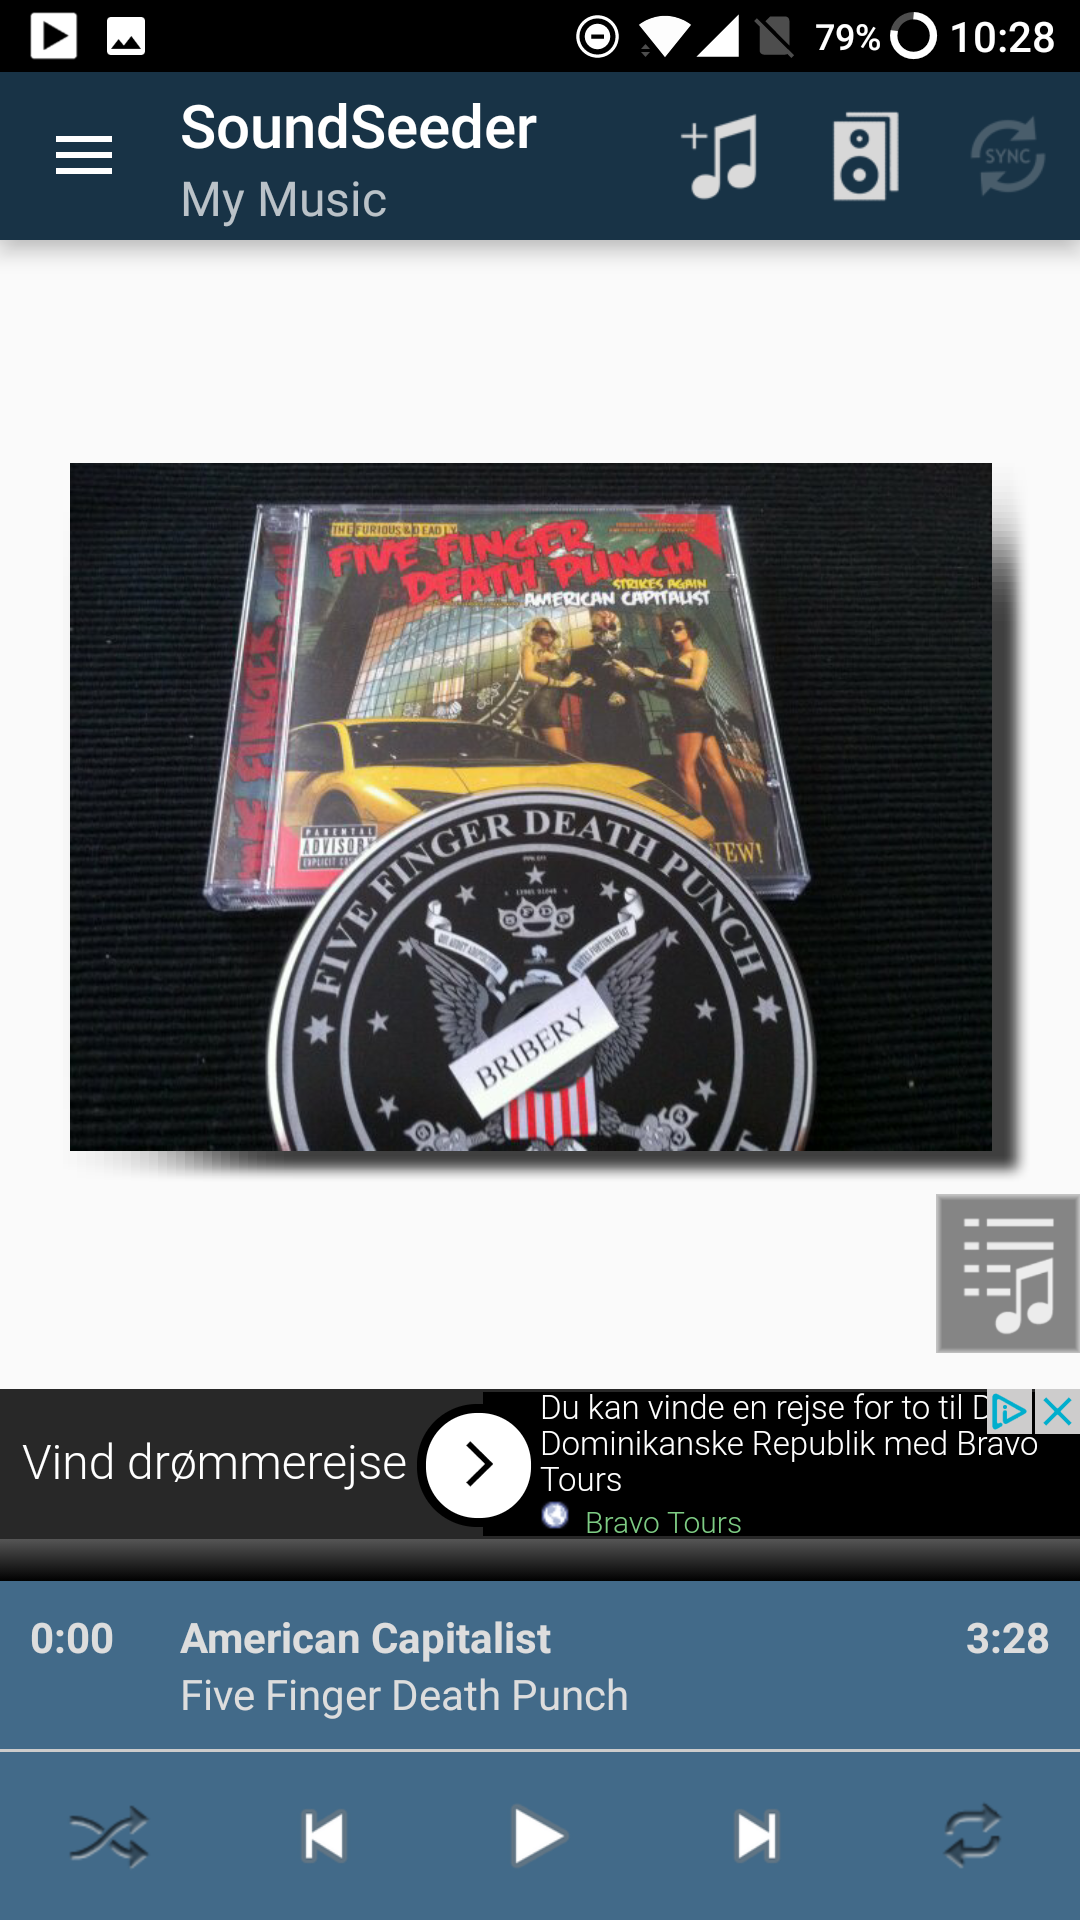
\includegraphics[width=0.65\textwidth]{img/sota/soundseeder.png}}
        \caption{When the app is opened.}\label{fig:soundseeder_screenshot}
    \end{subfigure}
    \hfill
    \begin{subfigure}[b]{0.45\textwidth}
        \footnotesize
        \centering
        \frame{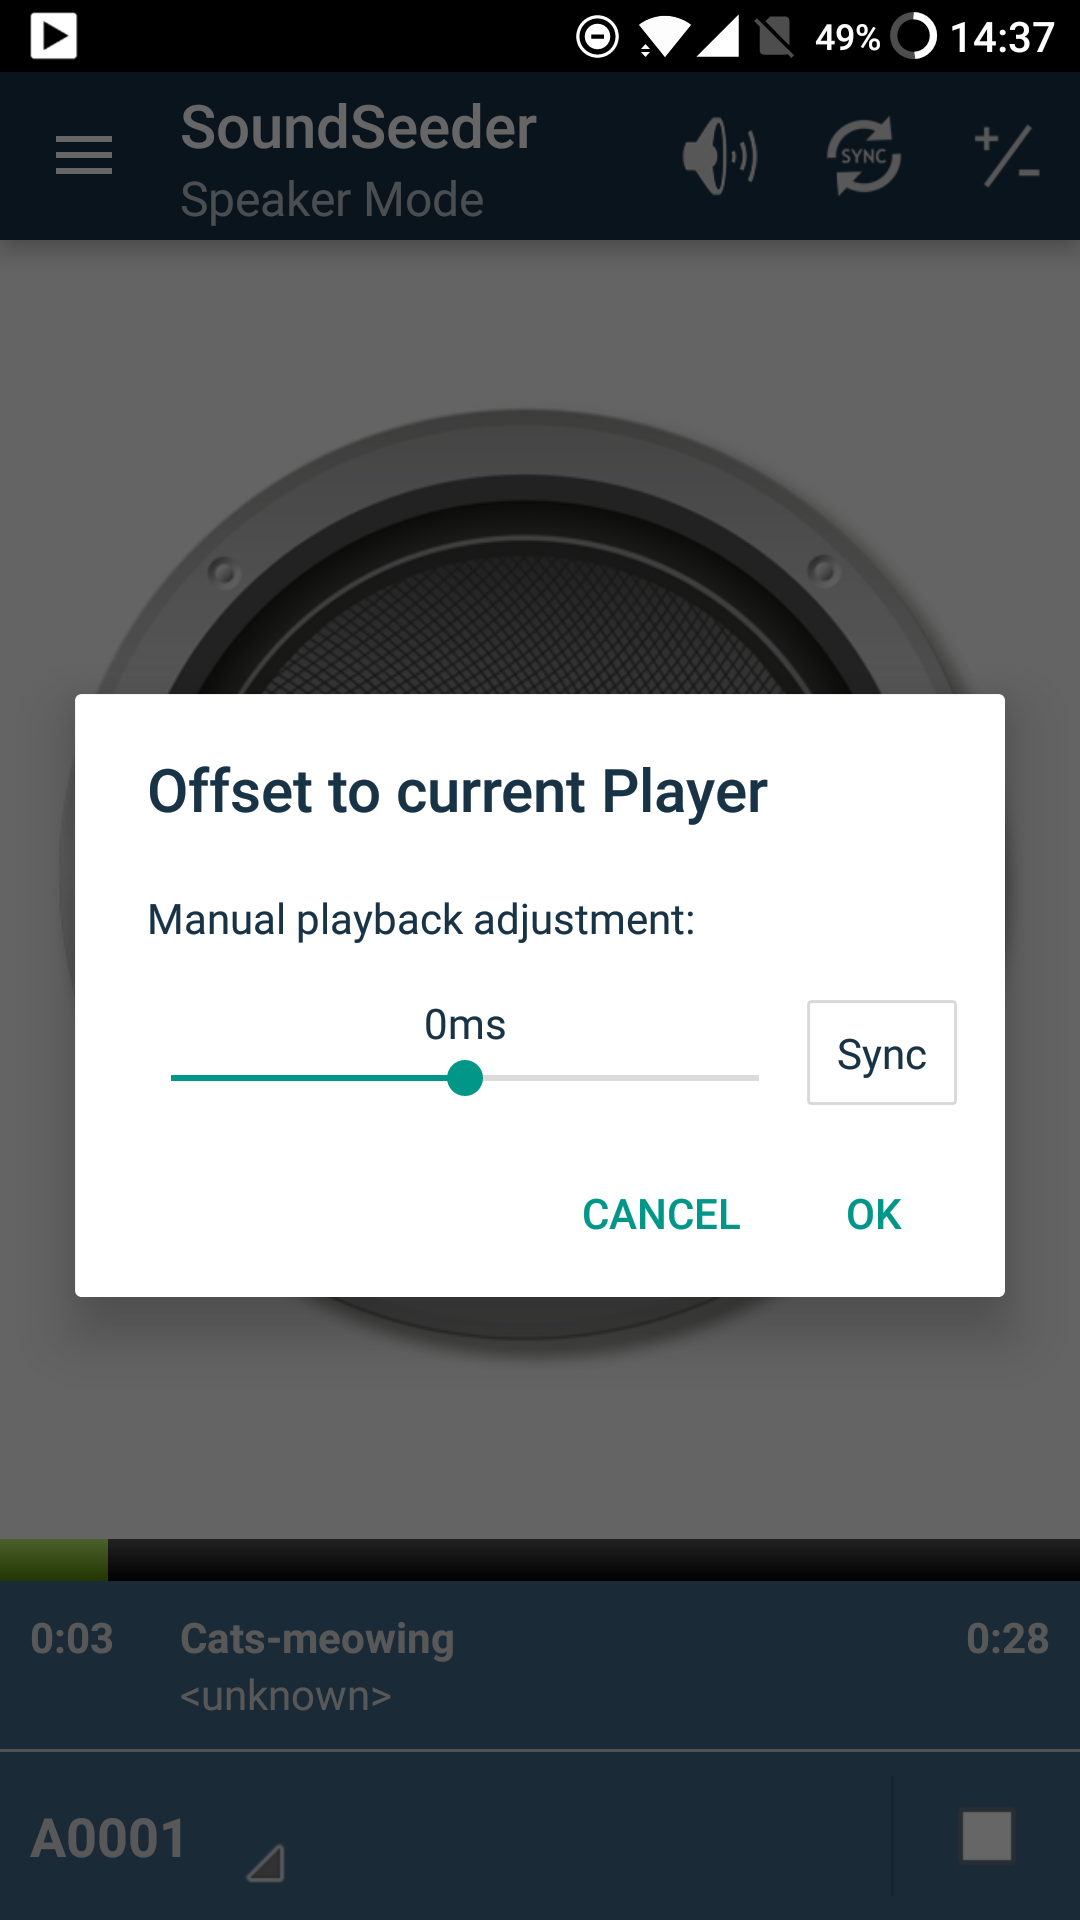
\includegraphics[width=0.65\textwidth]{img/sota/soundseeder_slider.png}}
        \caption{The synchronization slider.}\label{fig:soundseeder_slider}
    \end{subfigure}
    \caption{Screenshots from SoundSeeder}\label{fig:soundseeder_screenshots}
\end{figure}

\subsection{AmpMe}\label{subsec:ampme}
The second app is AmpMe\footnote{\url{http://www.ampme.com}}, made by Amp Me Inc.
The version of the app as of \formatdate{10}{2}{2017} is 5.1.1.
It supports Android 4.1 or newer and iOS 9.0 or newer.

In AmpMe the group of devices is called ``a party''.
When AmpMe is opened, it either displays the nearby parties or encourage you to create your own.
If a party is found nearby, you can join it as a slave and play the music of the master.
If no party is found, or you want to create your own, you can choose to start it by choosing between Spotify,
YouTube, your local music library, or SoundCloud as music source, as shown on \cref{fig:ampme_screenshot}.
When a source and music is chosen, a player appears with the music playing, and your device works as a master.

It is intuitive to join a party, or host one yourself and play music.
The interface is modern, minimalistic, and pleasant to use and look at.

In order to stream music from a master to slaves, AmpMe requires an Internet connection.
This means that the connected devices can be on WiFi, mobile data or another network, as long there is Internet access.

In AmpMe, the music is automatically synchronized upon party creation, but if there is an offset, it can be synchronized manually at each individual slave.
On \cref{fig:ampme_screenshot}, the slider to manually synchronize can be seen.
The slider goes from an offset of $-15$ to $+15$ arbitrary offset units, in increments of $1$.

AmpMe is free to use in both Google Play and the App Store.\cite{amp_faq, amp_play, amp_itunes}

\begin{figure}[h!]
    \centering
    \begin{subfigure}[b]{0.45\textwidth}
        \footnotesize
        \centering
        \frame{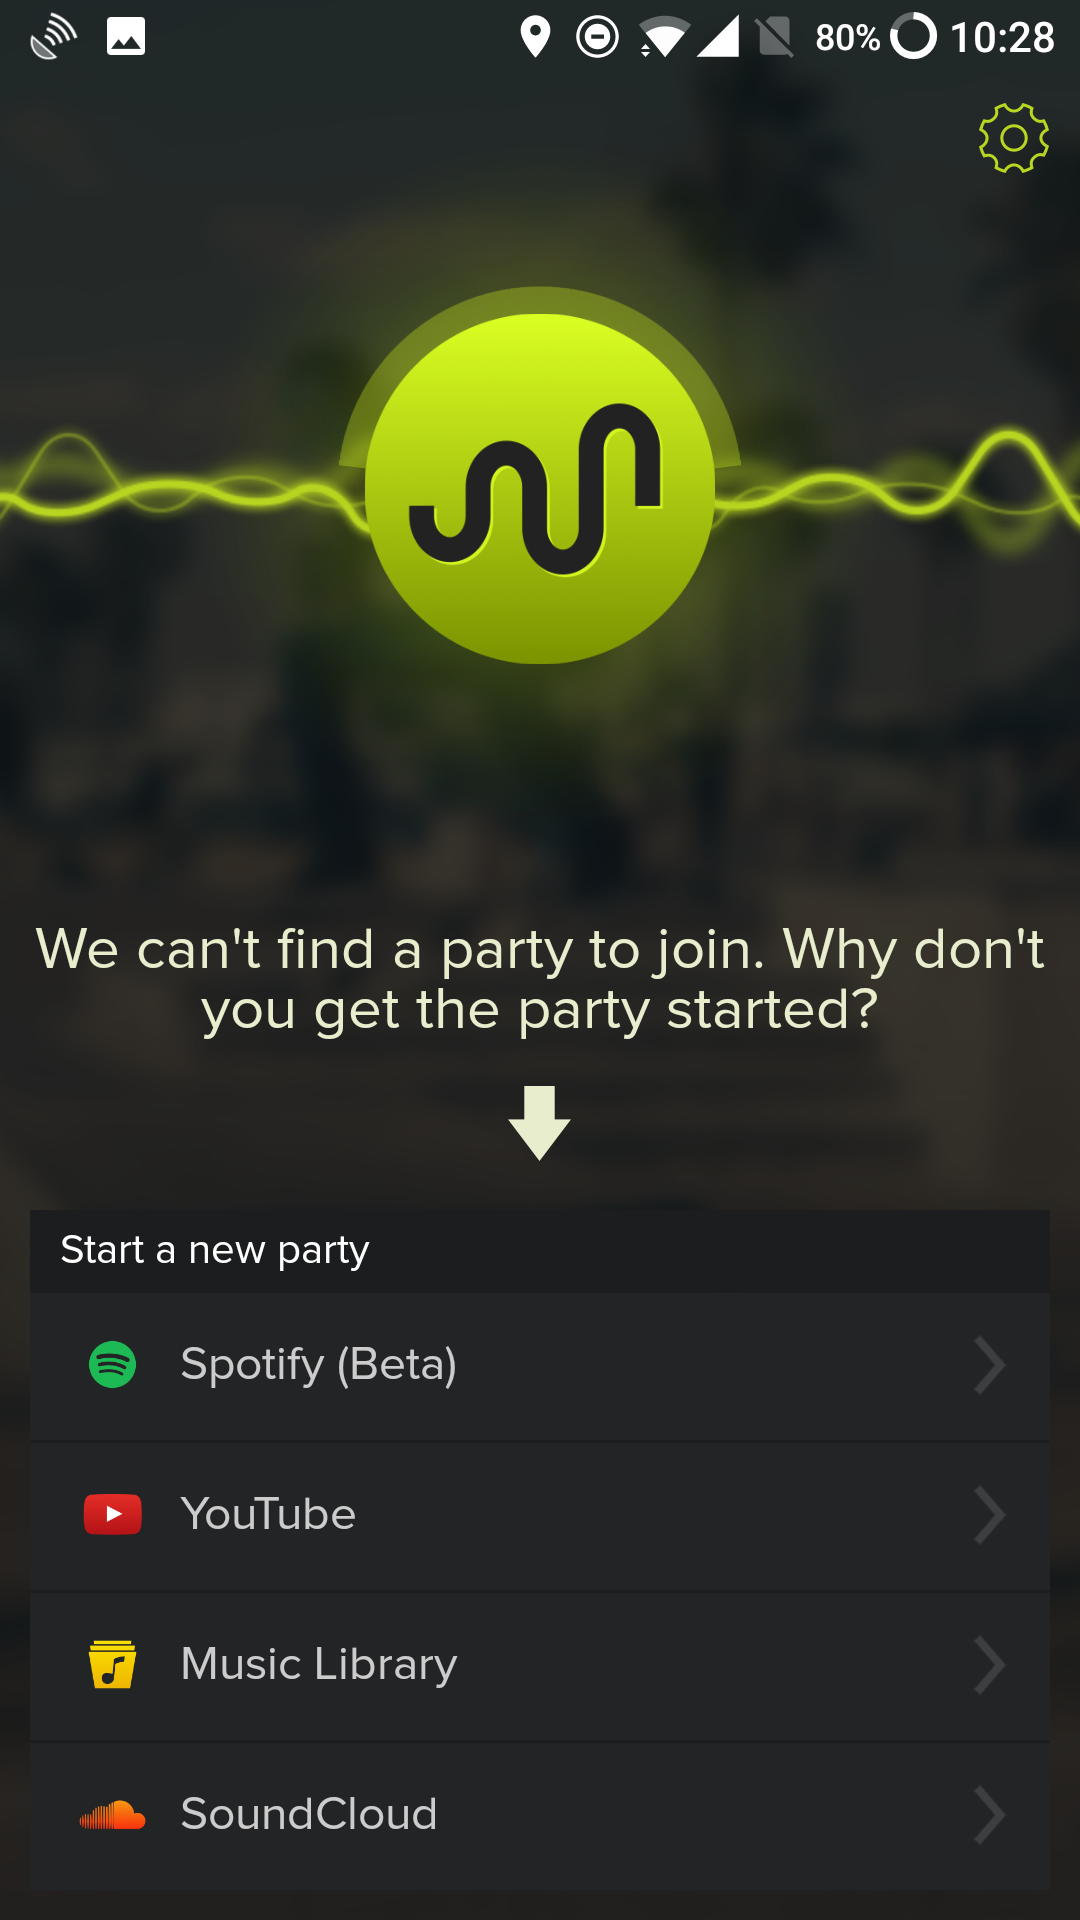
\includegraphics[width=0.65\textwidth]{img/sota/ampme.png}}
        \caption{When the app is opened.}\label{fig:ampme_screenshot}
    \end{subfigure}
    \hfill
    \begin{subfigure}[b]{0.45\textwidth}
        \footnotesize
        \centering
        \frame{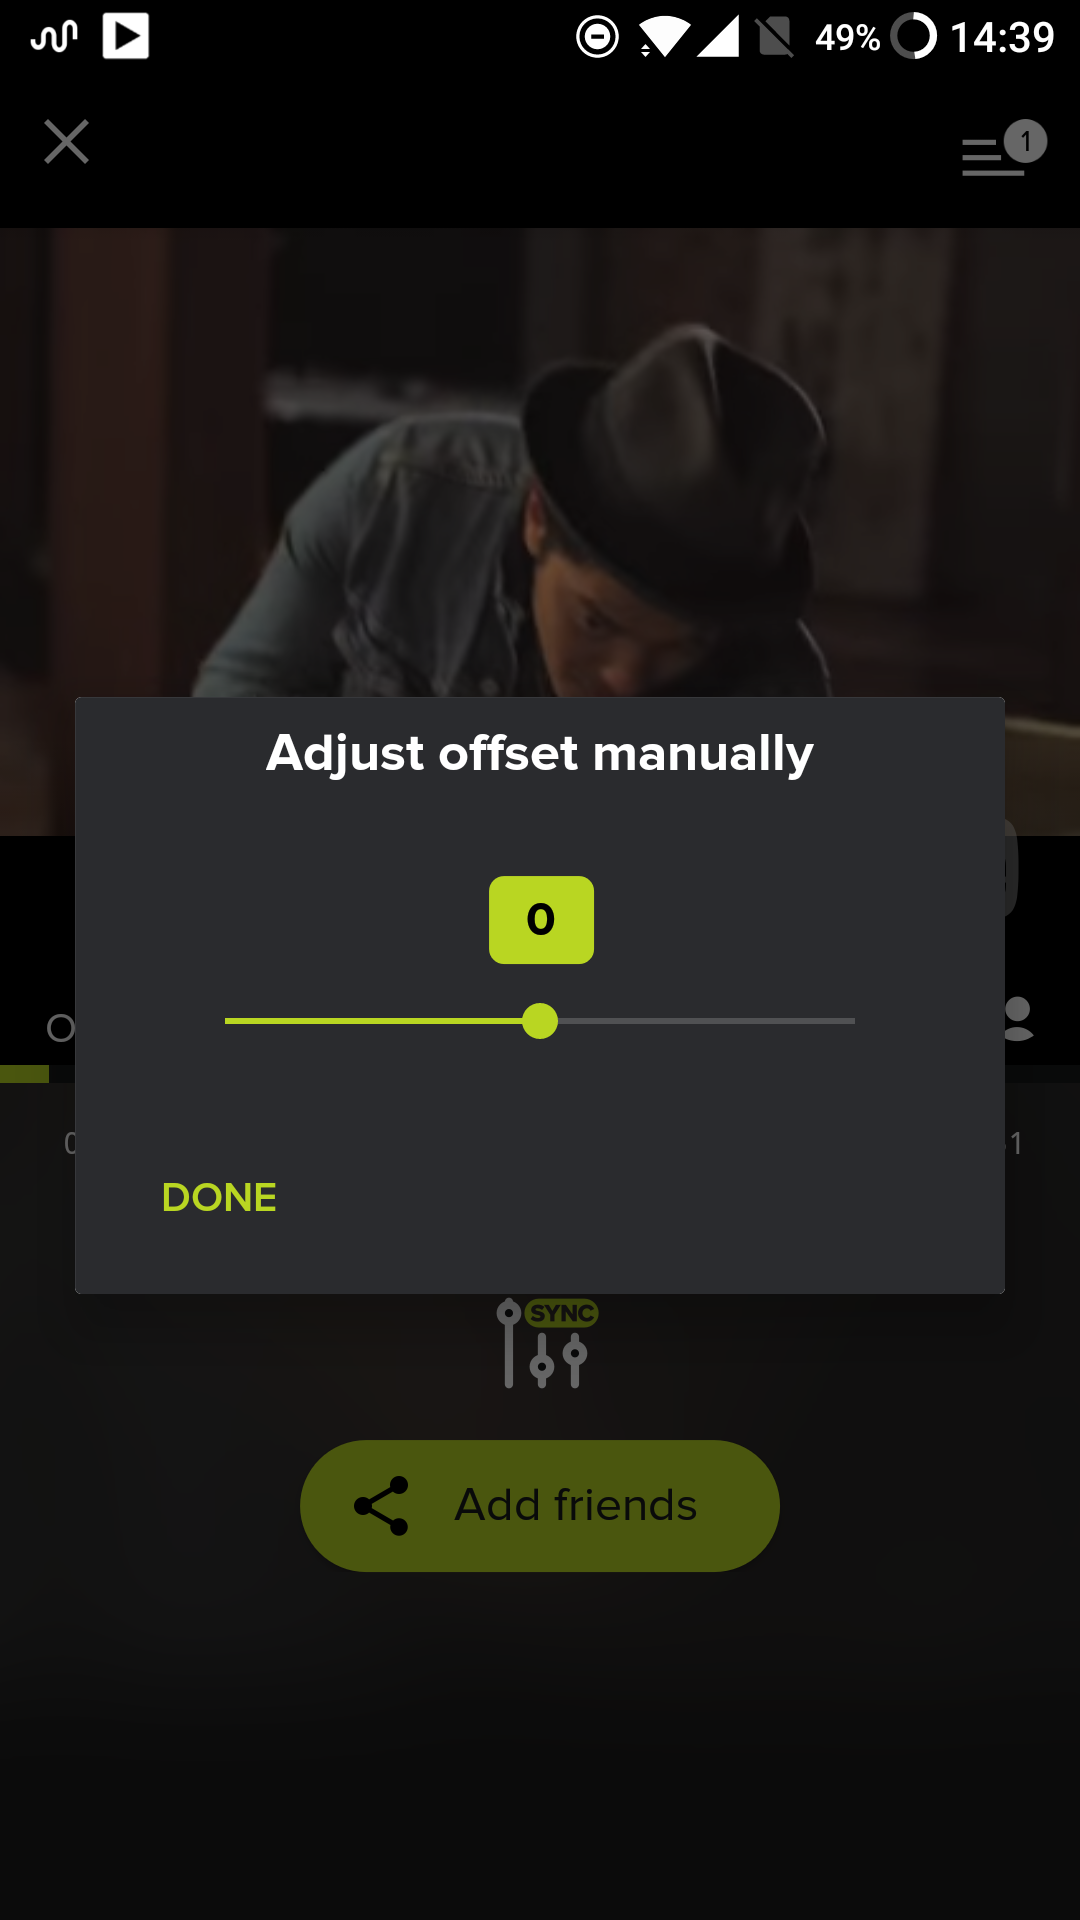
\includegraphics[width=0.65\textwidth]{img/sota/ampme_slider.png}}
        \caption{The synchronization slider.}\label{fig:ampme_slider}
    \end{subfigure}
    \caption{Screenshots from AmpMe}\label{fig:ampme_screenshots}
\end{figure}

\subsection{App Comparison}\label{ssec:app_comparison}
To determine what makes these apps state of the art, we look at their vital characteristics.
These vital characteristics are the user rating, last update date, supported devices, media sources, and connectivity options.
In \cref{tab:sota_comp}, a comparison of the apps can be seen.

\bigskip

SoundSeeder and AmpMe have their app ratings, Android support, YouTube and local media support in common.
AmpMe goes slightly beyond SoundSeeder when it comes to media support, by also supporting Spotify and SoundCloud.
Spotify has around 100 million users, which makes it an important source to support\cite{spotify_subscribers}.
SoundSeeder supports Google Music, and while they have not released any official user numbers it is expected to be lower than Spotify~\cite{googlem_subscribers}.

As for device support, AmpMe supports iOS devices, but SoundSeeder has a Java version which means that it supports all devices running Java.
Java support could prove advantageous in the case a computer was available as a media source, however this merely evens out the superior media support of Spotify in AmpMe.

As for connectivity, SoundSeeder supports streaming via WiFi or Android hotspot.
This may be an issue on larger and public networks where clients are often restricted from connecting with one another, although an Android hotspot can rectify the issue of a closed WiFi network.
AmpMe does not have this problem as it uses an Internet connection, however that does restrict one to internet and possible bandwidth issues.
As for the presented use cases in \cnameref{cha:establishing_use_cases}, either way of connecting the devices are acceptable.

Both SoundSeeder and AmpMe synchronizes automatically when the devices connect.
In the case that the synchronization becomes skewed, both apps have the possibility of manually synchronize and to set a synchronization offset.
The need for manual synchronization options could indicate that the automatic synchronization can at times be faulty, yet their creators find manual synchronization preferable to reconnecting.
The actual performance of the synchronization, in SoundSeeder and AmpMe will be tested in \cnameref{sec:sota_test}.

\begin{table}
\renewcommand\tabularxcolumn[1]{m{#1}}
\renewcommand{\arraystretch}{1.8}
    \small
    \begin{tabularx}{\textwidth}{XXX}\toprule
                                    & SoundSeeder                   & AmpMe                                                                     \\\midrule
        Rating (Out of 5)           & 3.9 Play Store                & 4.2 Play Store \newline 4.0 App Store                                     \\
        Latest update               & 11/11 2016                    & 30/1 2017                                                                 \\
        Supported \newline devices  & Android 4.1+ \newline Java Devices & Android 4.1+ \newline iOS 9.0+                                       \\
        Media source                & Google Music \newline YouTube \newline External devices \newline UPnP, DLNA \newline Online radio \newline Local media & Spotify \newline SoundCloud \newline YouTube \newline Local media  \\
        Connectivity                & WiFi \newline Android Hotspot & Internet                                                                  \\
        Pricing                     & 39.90 DKK                     & Free                                                                      \\\bottomrule
    \end{tabularx}
    \caption{Comparison between the apps as of the 13\textsuperscript{th} of February 2017.}\label{tab:sota_comp}
\end{table}
